\documentclass{article}
\usepackage[utf8]{inputenc}
\usepackage{hyperref}
\usepackage{graphicx}

\title{PigeonHole UGent Submission Platform User Manual}
\author{SEL group 1 2024}
\date{\today}

\begin{document}

\maketitle

\tableofcontents

\section{Introduction}
Welcome to the PigeonHole Ugent Submission Platform User Manual. This manual provides instructions for users, teachers, and administrators on how to effectively use the platform, step by step. The platform is designed to streamline the process of submitting, reviewing, and providing feedback on projects. It seeks to create a middle ground between being easy to use but also providing the necessary features for automatic feedback on big projects. As for now we only support UGent accounts to use the platform.

\section{Getting Started}
\subsection{Creating an Account}
Users can only login with their UGent account. If you do not have an account, please contact the administrator to create one for you.

\subsection{Logging In}
When acessing the platform, students will be prompted to log in with their UGent account. UGent uses OAuth2 for authentication, so you will be redirected to the UGent login page. After logging in, you will be redirected back to the platform.

\subsection{Changing language}
We support English and Dutch. You can change in the small dropdown menu in the top right corner of every page's topbar.

\subsection{Changing your profile picture}
By clicking on your name in the top right corner of the page, you can navigate to your profile page. Here you can change your profile picture by clicking on the image, selecting a new image, and clicking save.

\section{Student Section}

\begin{figure}[h]
    \centering
    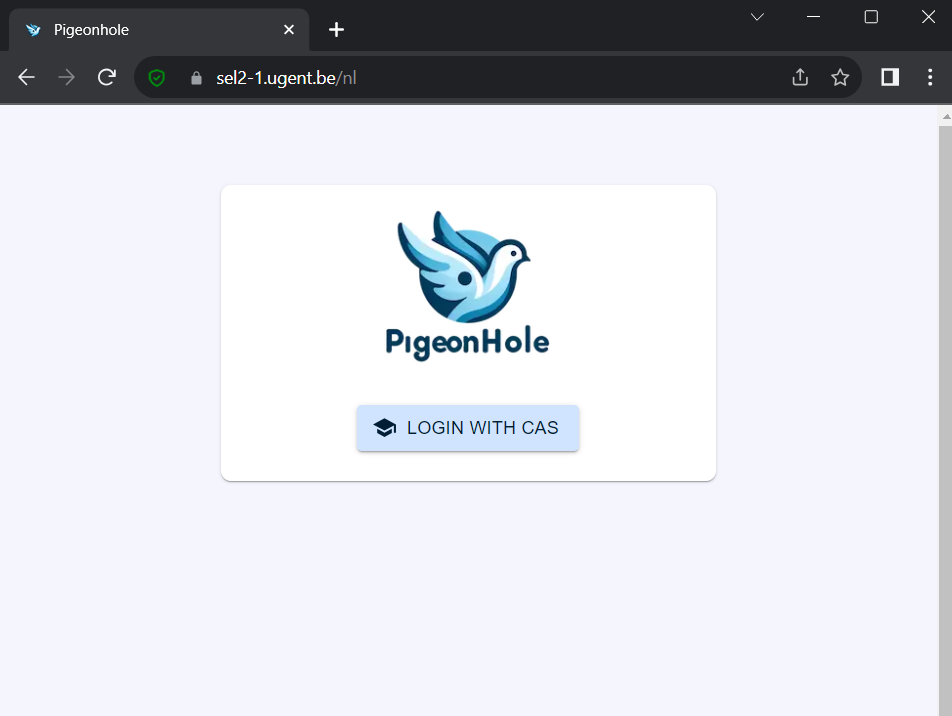
\includegraphics[width=0.5\textwidth]{images/login.png}
    \caption{Login Screen}
    \label{fig:login}
\end{figure}

\begin{figure}[h]
    \centering
    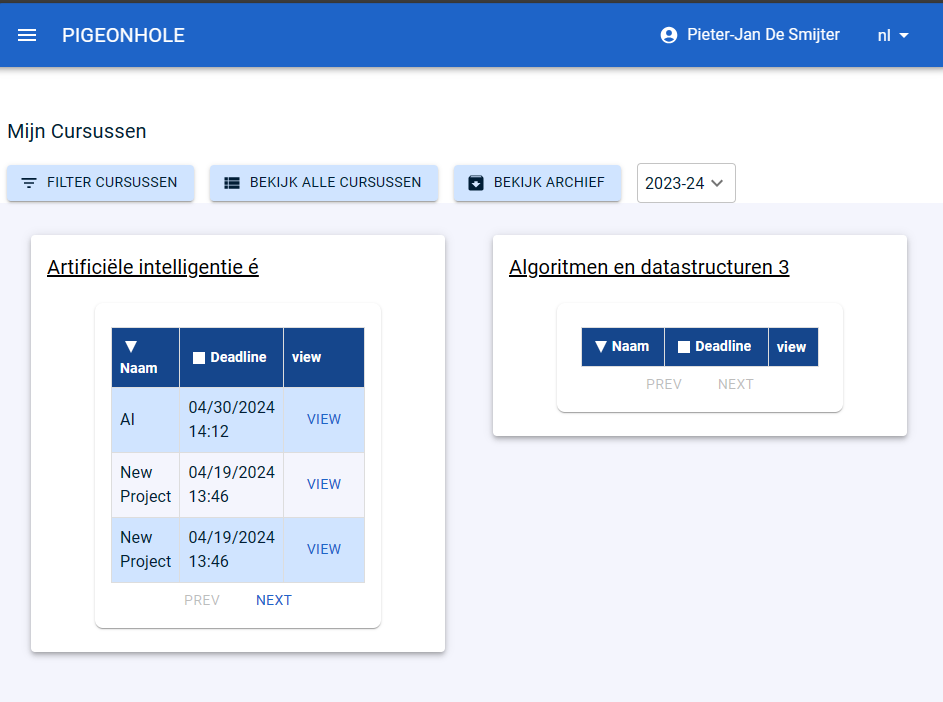
\includegraphics[width=0.5\textwidth]{images/home_page.png}
    \caption{Home page}
    \label{fig:home_page}
\end{figure}

\subsection{View your courses}

You can view all courses you are enrolled in and the projects that are available for submission central on the homepage. By clicking on a course title you can navigate to the course page, by clicking view project you can navigate to the project page.

\subsubsection{Archived courses}
Courses of previous years are archived and can be viewed by clicking on the "Archived courses" button.

\subsubsection{Filter courses}
You can filter the courses by typing in the search bar. (TO BE DONE)

\subsection{Join a new course}
There are two types of courses: public and private.
In case the course is private, you need to be invited by the teacher to join the course.

In case the course is public, you can eiter also be invited by the teacher or join the course yourself. 
To get a list of the public courses, click the "all open courses" button on the homepage.
On the "all open courses" page, you can see all public courses. By clicking on the "Join" button, you can join the course.

\subsection{Get an overview of the projects of a course}
On the home page, you can click on the course title to navigate to the course page. Here you can see all the projects of the course. You can see the status of the project and the deadline.
On the home page, you can also click on the "View project" button to navigate to a specific project page.
From the course page, you can also navigate to the project page by clicking on the "View project" button.

\subsection{Handing in a submission}
If you want to hand in a submission, you can do this by clicking on the "Make a submission" button on the project page. On the submit page, you can upload your files and submit them by dragging them into the dropzone or by clicking on the dropzone and selecting the files.

\subsection{Viewing feedback}
The automatic feedback will be immediately available after uploading the submission, even before you actually submit, on the submit page. Its possible to submit something that doesn't pass the automatic feedback, a red status will be shown with your submission.

\subsection{View your past submissions}
All your past submissions can be viewed on the project page.

\section{Teacher Section}
\subsection{Reviewing Projects}
Teachers can review submitted projects by following these steps:
\begin{enumerate}
    \item Log in to your teacher account.
    \item Navigate to the "Review Projects" or "Submitted Projects" section.
    \item View the list of submitted projects.
    \item Download project files for review.
\end{enumerate}

\subsection{Providing Feedback}
Teachers can provide feedback on submitted projects by:
\begin{enumerate}
    \item Downloading the project files.
    \item Reviewing the project.
    \item Providing written feedback or adding comments directly to the project files.
    \item Uploading the reviewed files.
    \item Optionally, adding automatic control or feedback code to the project.
\end{enumerate}

\section{Admin Section}
\subsection{Managing Users}
Admins can manage users by:
\begin{enumerate}
    \item Accessing the admin dashboard.
    \item Adding, editing, or removing user accounts.
    \item Resetting passwords or modifying user permissions.
\end{enumerate}

\subsection{Monitoring Projects}
Admins can monitor project submissions and teacher feedback by:
\begin{enumerate}
    \item Accessing the admin dashboard.
    \item Viewing project submission logs.
    \item Checking teacher feedback and comments.
\end{enumerate}


\section{A bit more information on the lists}
The lists of courses, projects, and submissions are paginated. You can navigate through the pages by clicking on the page number or the next/previous buttons.
Most lists are also filterable by typing in the search bar, and sortable columns have a white square in the header, you can click on this to sort the list by that column.
The square will become a triangle pointing up or down, indicating the direction of the sort.

\section{Troubleshooting}
If you encounter any issues while using the platform, please contact our support team for assistance. You can reach us via email at 'axel.lorreyne@ugent.be'.

\section{Conclusion}
This user manual covers the basic functionality of the Project Submission Platform for users, teachers, and administrators. For more information or assistance, please refer to the platform's help section or contact our support team.

\end{document}
